\documentclass[12pt,a4paper]{article}
\usepackage[utf8]{inputenc} %polskie znaki
\usepackage[T1]{fontenc}	%polskie znaki
\usepackage{amsmath}		%matematyczne znaczki :3
\usepackage{enumerate}		%Dodatkowe opcje do funkcji enumerate
\usepackage{geometry} 		%Ustawianie marginesow
\usepackage{graphicx}		%Grafika
\usepackage{wrapfig}		%Grafika obok textu
\usepackage{float}			%Allows H in fugire
\usepackage{hyperref}		%Allows hyperlinks
%\pagestyle{empty} 			%usuwa nr strony
\usepackage{todonotes}		%Todo notatki
\usepackage{lipsum}         %Lorem text
\usepackage{ntheorem}   	% for theorem-like environments
\usepackage{mdframed}   	% for framing
\usepackage{subcaption}		% subfigure (image placing)
\usepackage{pdfcomment}		% Komentarze (z bazowego pdf'a)
\usepackage{xparse}			% New commands with optional arguments
\usepackage{ifthen}			% If then - funkcje!
\usepackage{expl3}			% Deklarowanie zmiennych

\newgeometry{tmargin=2cm, bmargin=2cm, lmargin=2cm, rmargin=2cm} 

%Counter commands{
	\newcounter{counter} % Creates a new counter
	\setcounter{counter}{1} % Sets the counter to 5
	\newcommand{\counter}[1]{
		\arabic{#1} \stepcounter{#1} 
	}
	\newcommand{\counterreset}[1]{\setcounter{#1}{1}}
	%}

%Define styles{
	\theoremstyle{break}
	\theoreminframepreskip{0.5cm}
	\theoremheaderfont{\bfseries}
	\newmdtheoremenv[%
	linecolor=white,%
	innertopmargin=\topskip,
	shadowsize=0,%
	innertopmargin=5,%
	innerbottommargin=5,%
	leftmargin=10,%
	rightmargin=10,%
	backgroundcolor=gray!20,%
	innertopmargin=0pt,%
	ntheorem]{zad}{Zadanie}
	
	\mdfdefinestyle{zadanie}{
		linecolor=white,%
		innertopmargin=5,%
		innerbottommargin=5,%
		leftmargin=10,%
		rightmargin=10,%
		backgroundcolor=gray!20,%
		innertopmargin=8,
		innerbottommargin=8,
		skipabove = 5,
	}
	\mdfdefinestyle{wzor}{
		linecolor=cyan,%
		linewidth=2pt,%
		innertopmargin=8,
		innerbottommargin=8,
		leftmargin=10,%
		rightmargin=10,%
		backgroundcolor = white, 
		fontcolor = black,
		skipabove = 5,
		skipbelow = 5,
	}
	%}

%Zadania templatex%{
	\newcommand{\Wzor}[1]{
		\begin{mdframed}[style=wzor]
			\centering #1
		\end{mdframed}
	}
	\newcommand{\ZadanieTextowe}[1]{
		\begin{mdframed}[style=zadanie]
			\textbf{Zadanie \counter{counter} } \\
			#1
		\end{mdframed}
	}
	\newcommand{\Zadanie}[2]{
		\ZadanieTextowe{#1}
		#2
	}
	\newcommand{\ZadanieABCD}[6]{
		\ZadanieTextowe{#1}
		#2 \\\\
		\begin{tabular}{p{7cm} p{7cm}}
			\textbf{A. }#3&
			\textbf{B. }#4\\\\
			\textbf{C. }#5&
			\textbf{D. }#6\\
		\end{tabular}
	}
	\newcommand{\ZadanieABCDEF}[8]{
		\ZadanieTextowe{#1}
		#2 \\\\
		\begin{tabular}{p{7cm} p{7cm}}
			\textbf{A. }#3&
			\textbf{B. }#4\\\\
			\textbf{C. }#5&
			\textbf{D. }#6\\\\
			\textbf{E. }#7&
			\textbf{F. }#8\\\\
		\end{tabular}
	}
	\newcommand{\Zadanietwoxtwo}[5]{
		\ZadanieTextowe{#1}
		\begin{tabular}{p{7cm} p{7cm}}
			\textbf{a)} #2&
			\textbf{b)} #3\\\\
			\textbf{c)} #4&
			\textbf{d)} #5\\\\
		\end{tabular}
	}
	\newcommand{\Zadanietwoxthree}[7]{
		\ZadanieTextowe{#1}
		\begin{tabular}{p{7cm} p{7cm}}
			\textbf{a)} #2&
			\textbf{b)} #3\\\\
			\textbf{c)} #4&
			\textbf{d)} #5\\\\
			\textbf{e)} #6&
			\textbf{f)} #7\\\\
		\end{tabular}
	}
	\newcommand{\Zadanietwoxfour}[9]{
		\ZadanieTextowe{#1}
		\begin{tabular}{p{7cm} p{7cm}}
			\textbf{a)} #2&
			\textbf{b)} #3\\\\
			\textbf{c)} #4&
			\textbf{d)} #5\\\\
			\textbf{e)} #6&
			\textbf{f)} #7\\\\
			\textbf{g)} #8&
			\textbf{h)} #9\\\\
		\end{tabular}
	}
	%}


\begin{document}
	
	\begin{center}
		\LARGE Zadania na lekcje 1 - podstawy algebry
	\end{center}
	
	\Zadanietwoxtwo{Rozwiąż równania:}
	{$2(x-3)=3(x+5)$}
	{$4(x+4)-2(3x-5)=8$}
	{$2(x-3)-3(6+x)=6-(3+x)$}
	{$\frac{x-1}{2}+\frac{1}{4}(x-1)=9$}
	\Zadanietwoxthree{Rozwiąż nierówności:}
	{$3x+5(x-3)\geq 14-(x+4)$}
	{$2-x<x+7$}
	{$\frac{1}{3}(x+3)+\frac{x}{5} - x < 4 - \frac{x-3}{15}$}
	{$\frac{2x+5}{3}-\frac{x-7}{6}$> $\frac{1}{2}$}
	{$2(x-3)<\frac{2-x}{3}+\frac{3}{2}(x-5)$}
	{$\frac{1}{2}(x-3)-\frac{6+x}{3}<\frac{x}{6}$}
	\Zadanietwoxthree{Dla poniższych równań i nierówności przedstaw ich interpretację geometryczną, a następnie rozwiąż:}
	{$|x-3|=5$}{$|x+4|<4$}
	{$|x+5|=-2$}
	{$|x+6|>2\frac{1}{5}$}
	{$|2x-3|=6$}{$-|4-x|>-2$}
	

	\ZadanieTextowe{Rozpisz korzystając ze wzorów skróconego mnożenia:}
	\begin{enumerate}[a)] \begin{tabular}{p{5cm} p{5cm} p{5cm}} 
			\item $(x+2)^2$ & \vspace{0.25cm}\item$(x-3)^2$ &\vspace{0.25cm}\item $(2x+5)^2$\\
			\item $(x+2y)^2$ & \item $(3+2x)^2$ &\item $(5x+2)^2$\\
			\item $(-x-2)^2$ & \item $(-3y+7)^2$ &\item $(-5x+3)^2$\\
			\item $(x-2y)(x+2y)$ & \item $(3x+1)(3x-1)$ &\item $(4+5x)(5x-4)$\\
			\item $(x^2-4)(x^2+4)$ & \item $(4a+7b)(7b-4a)$ &\item $(-x-2y)(2y-x)$\\
	\end{tabular} \end{enumerate}
\newpage
	\Zadanietwoxthree{Rozpisz korzystając ze wzorów skróconego mnożenia:}
	{$(x+2y)^2+(x-2y)^2$}
	{$(3x-4)^2-(3x+4)^2$}
	{$(5x-3y)^2+(3x-5y)^2$}
	{$(x+\frac{1}{2}y)(x-\frac{1}{2}y)-(\frac{1}{2}y-x)(x+\frac{1}{2}y)$}
	{$(2\sqrt{2}-8)^2-(3\sqrt{3}+2\sqrt{2})^2$}
	{$(\sqrt{5}-2\sqrt{2})(2\sqrt{2}+\sqrt{5})-(4\sqrt{3}+2\sqrt{2})^2$}

	\ZadanieTextowe{
		Udowodnij, że liczba
		$$(x+1)^2+(x-1)^2$$
		jest podzielna przez 2, dla każdej liczby naturalnej x.
	}

	\ZadanieTextowe{
		Udowodnij, że liczba
		$$(x+4)^2+(x-3)^2-(x+4)^2-(x-1)^2$$
		jest podzielna przez 4, dla każdej liczby naturalnej x.
	}

	\ZadanieTextowe{
		Udowodnij, że suma dwóch kolejnych nieparzystych liczb naturalnych jest podzielna przez 4.
	}

	\ZadanieTextowe{
		Udowodnij, że suma dwóch kolejnych parzystych liczb naturalnych przy dzieleniu przez 4 daje resztę 2.
	}

	\ZadanieTextowe{
	Udowodnij, że liczba
	$$x^2+3x+2$$
	jest podzielna przez 2.
	}

	\Zadanietwoxtwo{Wykaż, że dla dowolnych liczb rzeczywistych x,y prawdziwe są nierówności:}
	{$x^2+2xy+3y^2\geq 0$}
	{$2x^2+25x^2\geq 10xy$}
	{$x^4y^2+2x^3y^3+x^2y^4\geq0$}
	{$\frac{3x^2}{4}+\frac{y^2}{3}-xy\geq0$}

	\newpage

	\begin{center}
	\LARGE Zbiór zadań - podstawy algebry
	\end{center}
	\Wzor{
		\begin{tabular}{p{7cm} p{7cm}}
			\centering$(a+b)^2=a^2+2ab+b^2$&
			\centering$(a-b)^2=a^2-2ab+b^2$\\
		\end{tabular}
	}
	\Wzor{
		$(a-b)(a+b)=a^2-b^2$
	}
	\Zadanietwoxfour{Rozwiąż równania i nierówności: \pdfcomment[timezone=+01'00',icon=Help,color=yellow]{Podpowiedź: Uważaj na minusy!}}
	{$\frac{x+2}{3}=\frac{x+1}{2}$}
	{$2x-3(x+6)=4x+2$}{$(x+3)^2-(x-2)^2=7$}
	{$4-2x<x-8$}
	{$\frac{3}{5}(x-1)-\frac{x-3}{2}\leq\frac{x-8}{10} $}
	{$\frac{x(x-1)}{4}-\frac{2x^2+1}{2}=-\frac{3}{4}x^2-0,25(x+2)$}
	{$3(2-4x)+2x\geq5(1-2x)$}
	{$-1\frac{2}{3}(x+6)\geq\frac{1}{6}(x+3)+0,5$}

	\ZadanieTextowe{Rozpisz korzystając ze wzorów skróconego mnożenia:}	
	\begin{enumerate}[a)] \begin{tabular}{p{5cm} p{5cm} p{5cm}} 
		\item $(9-4y)^2$ & \vspace{0.25cm}\item$(x-4)^2$ &\vspace{0.25cm}\item $(3x+1)^2$\\
		\item $(4+3e)^2$ & \item $(1-2x)^2$ &\item $(4x+8)^2$\\
		\item $(a-1)^2$ & \item $(6-3a)^2$ &\item $(3b-7x)^2$\\
		\item $(x-y)(x+y)$ & \item $(3x+4)(3x-4)$ &\item $(2+7x)(7x-2)$\\
		\item $(xy-5)(xy+5)$ & \item $(4a-6b)(6b+4a)$ &\item $(-x-4y)(4y-x)$\\
	\end{tabular} \end{enumerate}

	\Zadanietwoxthree{Rozpisz korzystając ze wzorów skróconego mnożenia:\pdfcomment[timezone=+01'00',icon=Help,color=yellow]{Podpowiedź: Uważaj na minusy przed nawiasami!}}
	{$5y^2-3(y+1)(y-1)$}{$(4+3y)(4-3y)-(4-y)^2$}
	{$(3x+1)(3x+1)+(1+5x)(1-5x)$}{$(x-7)^2-(4-2x)^2$}
	{$(\sqrt{2}+2)^2+(\sqrt{3}-3)^2$}{$(2-\sqrt{5})(2+\sqrt{5})-(2-\sqrt{5})^2$}
	\newpage
	\ZadanieTextowe{Usuń niewymierność z podanych wyrażeń:\pdfcomment[timezone=+01'00',icon=Help,color=yellow]{Podpowiedź: podpunty a,b,c wymnoz przez pierwiastek, natomiast pozostale wynóż ze wzoru skróconego mnożenia - 3 wzór}}
	
	\begin{enumerate}[a)] \begin{tabular}{p{5cm} p{5cm} p{5cm}} 
			\item \Large$\frac{1}{\sqrt{2}}$ & \vspace{0.25cm}\item\Large$\frac{4}{2\sqrt{2}}$ &\vspace{0.25cm}\item \Large$\frac{6\sqrt{2}}{\sqrt{3}}$\\
			\item \Large$\frac{1}{1+\sqrt{2}}$ & \item \Large$\frac{4}{\sqrt{5}-1}$ &\item \Large$\frac{2\sqrt{6}}{\sqrt{6}+2}$\\
			\item \Large$\frac{2+\sqrt{5}}{\sqrt{5}-1}$ & \item \Large$\frac{\sqrt{2}+3}{3-\sqrt{2}}$ &\item \Large$\frac{5+\sqrt{3}}{3+\sqrt{5}}$\\
	\end{tabular} \end{enumerate}
	\ZadanieABCD{Poniżej przedstawiono interpretację geometryczną w postaci przedziału pewnej nierówności:}{
	\begin{figure}[h]
		\centering
		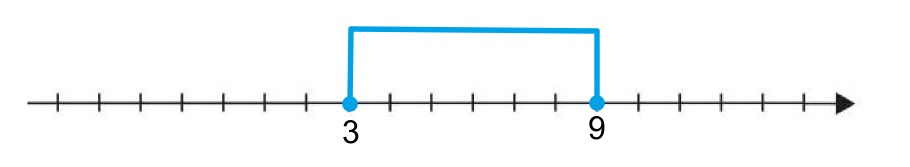
\includegraphics[scale=0.5]{z1_1.jpeg}
	\end{figure}	
	Nierówność opisującą ten przedział można opisać za pomocą:
	}{$|x+6|\leq3$}{$|x-6|\leq3$}{$|x+6|\geq3$}{$|x-6|\geq3$}

	\ZadanieABCD{Nierówność $|x-2|>4$ można przedstawić za pomocą przedziału:}{tresx}
	{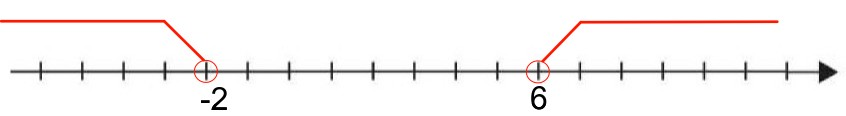
\includegraphics[width=6cm, height=1.3cm]{z1_2_1.jpeg}}
	{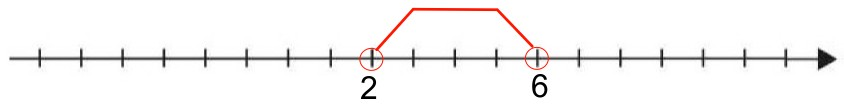
\includegraphics[width=6cm, height=1.3cm]{z1_2_2.jpeg}}
	{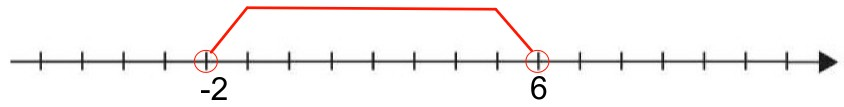
\includegraphics[width=6cm, height=1.3cm]{z1_2_3.jpeg}}
	{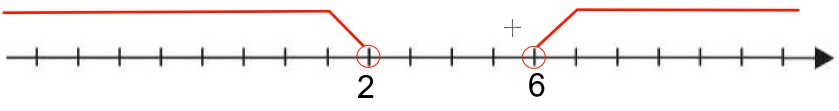
\includegraphics[width=6cm, height=1.3cm]{z1_2_4.jpeg}}

\ZadanieTextowe{Udowodnij, że liczba $$(2x+1)^2-(x+1)^2+x$$ jest podzielna przez 6. \pdfcomment[timezone=+01'00',icon=Help,color=yellow]{Podpowiedź: Rozpisz, a natępnie porównaj z zadaniem 5 i 7}}

\ZadanieTextowe{Udowodnij, że liczba $$5x^3-5x$$ jest podzielna przez 30. \pdfcomment[timezone=+01'00',icon=Help,color=yellow]{Podpowiedź: Wycianij przed nawias co sie da, a natepnie to co zostanie w nawiasie rozpisz ze wzoru skroconego mnozenia}}

\end{document}